
	\section{ACM/ICPC World Finals 2009}
		\subsection{ACM/ICPC World Finals 2009 B My Bad}
				\begin{wrapfigure}{r}{0.35 \textwidth}
					\centering
					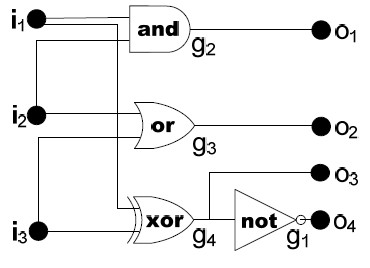
\includegraphics[width=0.3 \textwidth]{7.jpg}
					\caption{一个可能的门电路}
				\end{wrapfigure}
			\subsubsection{题目大意}
				给定一个门电路和若干次实验数据(输入,输出),判断是否
				\begin{enumerate}
					\item 全部元件工作正常;
					\item 某一个元件一直输出一,其他元件正常;
					\item 某一个元件一直输出零,其他元件正常;
					\item 某一个元件一直输出的值与正确的值相反,其他元件正常;或
					\item 有多种可能的故障,或只可能是多个元件的故障,或一个元件的多种故障,或无法判定其故障。
				\end{enumerate}
				
				门电路的数量 $N \le 19$,输入 $M \le 8$,输出 $K \le 19$。不同测试的输入两两不同。
			\subsubsection{算法讨论}
				直接枚举前四种情况,总共有 $(3 N + 1)$ 种可能(全部工作正常,某一元件有某一故障)。测试数最多 $2^M$ 种,代入  $(3 N + 1)$ 种可能中依次检验。若\emph{只有}某一种可能符合要求,那么答案就是该种可能;否则答案为最后一种情况。
				
				模拟逻辑电路时,需先拓扑排序,再计算。
			\subsubsection{时空复杂度}
				
				时间复杂度 $\mathcal{O}\left(N2^MN\right)$。
					
				空间复杂度 $\mathcal{O}\left(N 2^M(M + N)\right)$。
		\newpage
		\subsection{ACM/ICPC World Finals 2009 C The Return of Carl}
				\begin{wrapfigure}{r}{0.35 \textwidth}
					\centering
					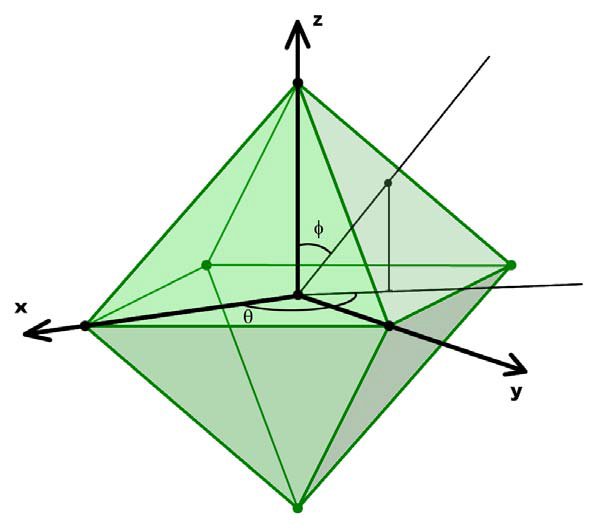
\includegraphics[width=0.3 \textwidth]{8.png}
					\caption{题目中的球坐标系}\label{09c1}
					\vskip-5em
				\end{wrapfigure}
			\subsubsection{题目大意}
				一个正八面体表面上有两点,问从一点经表面到达另一点的最短距离。
				
				坐标使用如图 \ref{09c1} 的球坐标系描述。
			\subsubsection{算法讨论}
				根据正八面体的对称性,可以将某一点旋转,翻转到第一卦限$(x, y, z > 0)$。根据另一个点的卦限分情况讨论。
				
				若另一点位于
				
				\begin{description}
					\item[第一卦限, \Rmnum{1}, $(+, +, +)$] 显然就是两点间的直线距离。
					\item[第二卦限, \Rmnum{2}, $(-, +, +)$] 将八面体一二卦限的面展开为平面,可以证明(暴力搜索)展开后两点的距离就是答案。
					\item[第三卦限, \Rmnum{3}, $(-, -, +)$] 将八面体一二三四卦限的面展开为平面,注意此处两个 \Rmnum{3} 的位置都有可能成为答案,同样可以证明展开后两点的距离就是答案。
					\item[第四卦限, \Rmnum{4}, $(+, -, +)$] 类似 第二卦限, \Rmnum{2}, $(-, +, +)$。
					\item[第五卦限, \Rmnum{5}, $(+, +, -)$] 类似 第二卦限, \Rmnum{2}, $(-, +, +)$。
					\item[第六卦限, \Rmnum{6}, $(-, +, -)$] 类似 第三卦限, \Rmnum{3}, $(-, -, +)$,有两个可能成为答案的位置。
				\begin{figure}[htb]
				\centering
				\definecolor{ffccww}{rgb}{1,0.8,0.4}
\begin{tikzpicture}[line cap=round,line join=round,>=triangle 45,x=1.0cm,y=1.0cm]
\fill[color=ffccww,fill=ffccww,fill opacity=0.25] (0,1.73) -- (1,0) -- (-1,0) -- cycle;
\node[color=ffccww] at (0, 1.73/3) {\Rmnum{1}};
\node[color=ffccww] at (1, 2 * 1.73/3) {\Rmnum{2}};
\node[color=ffccww] at (- 1, 2 * 1.73/3) {\Rmnum{4}};
\node[color=ffccww] at (1, 4 * 1.73/3) {\Rmnum{3}};
\node[color=ffccww] at (- 1, 4 * 1.73/3) {\Rmnum{3}};
\node[color=ffccww] at (2, 5 * 1.73/3) {\Rmnum{7}};
\node[color=ffccww] at (- 2, 5 * 1.73/3) {\Rmnum{7}};
\node[color=ffccww] at (2, 1.73/3) {\Rmnum{6}};
\node[color=ffccww] at (-2, 1.73/3) {\Rmnum{8}};
\node[color=ffccww] at (3, 2 * 1.73/3) {\Rmnum{7}};
\node[color=ffccww] at (- 3, 2 * 1.73/3) {\Rmnum{7}};
\node[color=ffccww] at (- 0, - 1  * 1.73/3) {\Rmnum{5}};
\node[color=ffccww] at (1, - 2  * 1.73/3) {\Rmnum{6}};
\node[color=ffccww] at (- 1, - 2  * 1.73/3) {\Rmnum{8}};
\node[color=ffccww] at (1, - 4  * 1.73/3) {\Rmnum{7}};
\node[color=ffccww] at (- 1, - 4  * 1.73/3) {\Rmnum{7}};
\fill[color=ffccww,fill=ffccww,fill opacity=0.25] (0,1.73) -- (-2,1.73) -- (-1,0) -- cycle;
\fill[color=ffccww,fill=ffccww,fill opacity=0.25] (0,1.73) -- (1,0) -- (2,1.73) -- cycle;
\fill[color=ffccww,fill=ffccww,fill opacity=0.25] (-3,0) -- (-2,1.73) -- (-1,0) -- cycle;
\fill[color=ffccww,fill=ffccww,fill opacity=0.25] (3,0) -- (1,0) -- (2,1.73) -- cycle;
\fill[color=ffccww,fill=ffccww,fill opacity=0.25] (-3,0) -- (-2,1.73) -- (-4,1.73) -- cycle;
\fill[color=ffccww,fill=ffccww,fill opacity=0.25] (3,0) -- (4,1.73) -- (2,1.73) -- cycle;
\fill[color=ffccww,fill=ffccww,fill opacity=0.25] (0,1.73) -- (-2,1.73) -- (-1,3.46) -- cycle;
\fill[color=ffccww,fill=ffccww,fill opacity=0.25] (-3,3.46) -- (-2,1.73) -- (-1,3.46) -- cycle;
\fill[color=ffccww,fill=ffccww,fill opacity=0.25] (0,1.73) -- (1,3.46) -- (2,1.73) -- cycle;
\fill[color=ffccww,fill=ffccww,fill opacity=0.25] (3,3.46) -- (1,3.46) -- (2,1.73) -- cycle;
\fill[color=ffccww,fill=ffccww,fill opacity=0.25] (0,-1.73) -- (1,0) -- (-1,0) -- cycle;
\fill[color=ffccww,fill=ffccww,fill opacity=0.25] (0,-1.73) -- (-2,-1.73) -- (-1,0) -- cycle;
\fill[color=ffccww,fill=ffccww,fill opacity=0.25] (0,-1.73) -- (-2,-1.73) -- (-1,-3.46) -- cycle;
\fill[color=ffccww,fill=ffccww,fill opacity=0.25] (0,-1.73) -- (1,0) -- (2,-1.73) -- cycle;
\fill[color=ffccww,fill=ffccww,fill opacity=0.25] (0,-1.73) -- (1,-3.46) -- (2,-1.73) -- cycle;
\draw [color=ffccww] (0,1.73)-- (1,0);
\draw [color=ffccww] (1,0)-- (-1,0);
\draw [color=ffccww] (-1,0)-- (0,1.73);
\draw [color=ffccww] (0,1.73)-- (-2,1.73);
\draw [color=ffccww] (-2,1.73)-- (-1,0);
\draw [color=ffccww] (-1,0)-- (0,1.73);
\draw [color=ffccww] (0,1.73)-- (1,0);
\draw [color=ffccww] (1,0)-- (2,1.73);
\draw [color=ffccww] (2,1.73)-- (0,1.73);
\draw [color=ffccww] (-3,0)-- (-2,1.73);
\draw [color=ffccww] (-2,1.73)-- (-1,0);
\draw [color=ffccww] (-1,0)-- (-3,0);
\draw [color=ffccww] (3,0)-- (1,0);
\draw [color=ffccww] (1,0)-- (2,1.73);
\draw [color=ffccww] (2,1.73)-- (3,0);
\draw [color=ffccww] (-3,0)-- (-2,1.73);
\draw [color=ffccww] (-2,1.73)-- (-4,1.73);
\draw [color=ffccww] (-4,1.73)-- (-3,0);
\draw [color=ffccww] (3,0)-- (4,1.73);
\draw [color=ffccww] (4,1.73)-- (2,1.73);
\draw [color=ffccww] (2,1.73)-- (3,0);
\draw [color=ffccww] (0,1.73)-- (-2,1.73);
\draw [color=ffccww] (-2,1.73)-- (-1,3.46);
\draw [color=ffccww] (-1,3.46)-- (0,1.73);
\draw [color=ffccww] (-3,3.46)-- (-2,1.73);
\draw [color=ffccww] (-2,1.73)-- (-1,3.46);
\draw [color=ffccww] (-1,3.46)-- (-3,3.46);
\draw [color=ffccww] (0,1.73)-- (1,3.46);
\draw [color=ffccww] (1,3.46)-- (2,1.73);
\draw [color=ffccww] (2,1.73)-- (0,1.73);
\draw [color=ffccww] (3,3.46)-- (1,3.46);
\draw [color=ffccww] (1,3.46)-- (2,1.73);
\draw [color=ffccww] (2,1.73)-- (3,3.46);
\draw [color=ffccww] (0,-1.73)-- (1,0);
\draw [color=ffccww] (1,0)-- (-1,0);
\draw [color=ffccww] (-1,0)-- (0,-1.73);
\draw [color=ffccww] (0,-1.73)-- (-2,-1.73);
\draw [color=ffccww] (-2,-1.73)-- (-1,0);
\draw [color=ffccww] (-1,0)-- (0,-1.73);
\draw [color=ffccww] (0,-1.73)-- (-2,-1.73);
\draw [color=ffccww] (-2,-1.73)-- (-1,-3.46);
\draw [color=ffccww] (-1,-3.46)-- (0,-1.73);
\draw [color=ffccww] (0,-1.73)-- (1,0);
\draw [color=ffccww] (1,0)-- (2,-1.73);
\draw [color=ffccww] (2,-1.73)-- (0,-1.73);
\draw [color=ffccww] (0,-1.73)-- (1,-3.46);
\draw [color=ffccww] (1,-3.46)-- (2,-1.73);
\draw [color=ffccww] (2,-1.73)-- (0,-1.73);
\end{tikzpicture}
				\caption{正八面体的展开图}\label{09c2}
				\end{figure}

					\item[第七卦限, \Rmnum{7}, $(-, -, -)$] 最复杂的一种情况,需要将整个多面体都展开。总共有六个可能的位置,如图  \ref{09c2}。
					\item[第八卦限, \Rmnum{8}, $(+, -, -)$] 类似 第三卦限, \Rmnum{3}, $(-, -, +)$,有两个可能成为答案的位置。
				
				\end{description}
				
				
				至于计算极坐标对应的点在展开图上的位置,可以先计算其在三维坐标系中的位置,方法是解方程

				\begin{align}
					\left\{\begin{array}{rcl}
							x &= &r \sin\theta \cos\phi \\
							y &  =&r \sin\theta \sin\phi \\
							z & =& r \cos\theta\\
							|x| + |y| + |z| & =&  1
						\end{array}
					\right.
				\end{align}
				随后确定其所在平面在展开图的\emph{线性}映射关系,从而计算出我们需要的值。
			\subsubsection{时空复杂度}
				
				时间复杂度 $\mathcal{O}\left(1\right)$。
					
				空间复杂度 $\mathcal{O}\left(1\right)$。
		\newpage
		\subsection{ACM/ICPC World Finals 2009 D Conduit Packing}
			\subsubsection{题目大意}
				四个实心圆柱,直径 $d_{1}, d_2, d_3, d_4$已知,高度为单位长度。试用一个高度为单位长度,直径 $d$ 尽量小的圆柱容器,使得四个实心圆柱均能同时放入其内。
				\begin{figure}[htb]
					\centering
					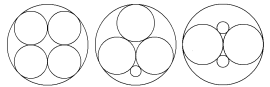
\includegraphics[width=0.5 \textwidth]{9.png}
					\caption{放置方法}
				\end{figure}
				
			\subsubsection{算法讨论}
				如果 $d$ 是合法的解,那么更大的解 $d + \Delta, \Delta > 0$ ,其仍然合法。故可先二分答案,检查某个特定的 $d$ 是否合法。	
				
				不妨枚举放入的顺序,设 $d_1, d_2, d_3, d_4 $ 先后放入其中。
				
				如果 $d < d_1$ 那么显然这个解是不合法的。否则可以贪心的将其放在容器的边缘。随后依次将后面的圆,与前面的某两个圆相切地,不重合地放入内。具体与哪两个圆相切,需要枚举。如果能够放下四个圆,那么返回有解。如果不行,更改放入的顺序继续搜索。如果无论如何都不行,那么只能返回无解。
				
				贪心的正确性可用调整法粗略地证明。如果某一个圆只与一个圆相切,或者完全不相切,那么在不与其他圆重合的情况下,稍稍移动一点,就可以与至少两个圆重合。
				
				配合二分搜索,即可求知答案。
			\subsubsection{时空复杂度}
				
				时间复杂度 $\mathcal{O}\left(k\right)$。$k$ 是二分次数,与精度相关。由于只有四个圆,搜索出来的情况数非常有限,并且是常数,故没有写入时间复杂度上限。
					
				空间复杂度 $\mathcal{O}\left(1\right)$。
		\newpage
		\subsection{ACM/ICPC World Finals 2009 G House of Cards}
			\subsubsection{题目大意}
				一个扑克游戏。洗好一碟 $2 M$ 张牌。牌有点数(1 到 13)和花色(赤黑)之分。先用八张牌按顺序摆成图 \ref{2009G} 所示的样子,作为起始局面。随后两个人(赤黑)顺次抽牌。第一张牌的颜色决定先手。每个人可以
				\begin{enumerate}
					\item 保留当前拿着的牌,并视之为保留牌(要在手中没有保留的牌时);
					\item 在两张构成谷的牌上横着搭一张,变为平的;如果手中还有有一张牌,则视之为保留牌;或者
					\item  在平的地方用保留牌和抽到的牌搭一个峰。
				\end{enumerate}
				每次执行后两个操作形成三角后,对应的三张牌的点数之和将会作为分数,加入到这三张牌中,最多的颜色对应的人上。分多的人获胜。
				
				两人均使用最优策略,试问赤黑两人谁能获胜。
				
				$M \le 13$。
				\begin{figure}[htb]
					\centering
					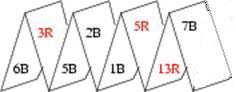
\includegraphics[width=0.3 \textwidth]{10.png}
					\caption{可能的开始局面}\label{2009G}
				\end{figure}
				
			\subsubsection{算法讨论}
				大方向是 博弈搜索 与 $\mathrm{\alpha}$-$\mathrm{\beta}$ 剪枝。将结果视为黑的得分减去赤的得分,那么黑就会最大化该值,赤最小化该值,套用博弈搜索即可知道结果。
				
				讨论下博弈搜索的细节。最多有 $2M$ 个牌位,其中 $8$ 个已固定,那么剩余的牌会产生远远不足 $(2M - 8 + 1)^2 \cdot(2M - 8)! \le 19^2 18!$ 的状态,配合$\mathrm{\alpha}$-$\mathrm{\beta}$ 剪枝,状态数会更少。应该可以通过测试。
			
			\subsubsection{时空复杂度}
				忽略 $\mathrm{\alpha}$-$\mathrm{\beta}$ 剪枝,时间复杂度 $\mathcal{O}\left(M^2 \cdot (2M)!\right)$。 $\mathrm{\alpha}$-$\mathrm{\beta}$ 剪枝非常有效,实际情况远远不足该上限。
					
				空间复杂度 $\mathcal{O}\left(1\right)$。
		\newpage
		\subsection{ACM/ICPC World Finals 2009 H The Ministers’ Major Mess}
			\subsubsection{题目大意}
				有 $N$ 项决议,$M$ 个人对其中 $k, k \le 4$ 项决议投票(同意或反对)。请确定哪些决议需要实施,哪些协议不许实施,使得每个人的投票中,有\emph{超过}半数的项目都得以满足。需要确定哪些决议必须通过,那些决议不许通过,哪些决议可通过可不通过;或者直接返回无解。			
				
				$N \le 100, M \le 500$。
			\subsubsection{算法讨论}	
				类似于  \textit{POI 2001 Peaceful Commission },转为 $2\text{-SAT}$。
				
				具体地,对于 $k = 1, 2$ 的人,其投票的内容是板上钉钉的事,故对于每一票 $x$,添加条件 $\bar{x} \rightarrow x$。$\rightarrow$ 表示蕴含,$A \rightarrow B = \neg A \vee B$。$\bar{x}$ 是 ${x}$ 的对立事件。
				
				对于 $k = 3, 4$ 的人,至多有一票被违背,故设其投票 $x_1, x_2, \ldots, x_k$,则添加条件
$\bigwedge_{i \ne j} (\bar{x_i} \rightarrow x_j) = 1$。
				
				此 SAT 问题的解与原问题的解一一对应。根据  $2\text{-SAT}$  的解法和相关推论,建好图后,若某 $\bar{x}, x$ 位于同一强连通块,则问题无解。否则肯定是有解的。
				
				若对于某一决议 $x$,$x \rightarrow \bar{x}$,即对应结点存在有向路径,那么显然 $x$ 不能被通过;反之 若 $x \leftarrow \bar{x}$,则其必须被通过。
				
				而如果 $x, \bar{x}$ 间无任何逻辑关系(对应点根本不连通),则 $x$ 可通过可不通过,因为考虑到求解 SAT 问题时,会先拓扑排序,然后根据拓扑序先入为主地确定哪些结点被选择。既然目前对应点根本不连通,则其都有可能在拓扑序中靠前地被选择,故都有可能构造出一个可能的合法解。
				
				根据以上的分析,求两点间的连通性,可判定出答案。
			\subsubsection{时空复杂度}
				时间复杂度 $\mathcal{O}\left(N(N + M)\right)$。
					
				空间复杂度 $\mathcal{O}\left(N + M\right)$。
		\newpage
		\subsection{ACM/ICPC World Finals 2009 I Struts and Springs}
			\subsubsection{题目大意}
				问题描述了一个在嵌套的窗口中,主窗口尺寸了发生改变后,子窗口的尺寸的变化的棍棒弹簧响应机制。
				
				对于每个子窗口,其向父窗口在对应的四个边缘上连接了四条线,同时此窗口的底部和顶部,左侧和右侧也分别连了线。每条线均可能是棍棒或弹簧。外层窗口移动时,内层窗口的变化服从物理原理,即棍棒的长度不会变化,而弹簧的变化服从胡克定律,即同一方向的弹簧等比例伸缩。如果某一方向上三条线都是棍棒,则最上或最右的棍棒变为弹簧。
				
				给定窗口的初始位置,请模拟这个响应机制的结果。
				
				窗口数 $N \le 100$,尺寸变化操作次数 $\le 100$。.
				
			\subsubsection{算法讨论}	
				先需要根据窗口位置,确定窗口父子关系。简单的 $\mathcal{O}\left(N^2\right)$ 的暴力就可以解决。先枚举一个窗口,则包围了他的,且面积最小的就是其父窗口。
				
				随后根据题目中表述的模型直接模拟即可。注意到除了主窗口外,其他的窗口左上角的坐标还会有偏移,在递归时须考虑到。
			
			
			\subsubsection{时空复杂度}
				时间复杂度 $\mathcal{O}\left(N^2 + NM\right)$。
					
				空间复杂度 $\mathcal{O}\left(N\right)$。
		\newpage
		\subsection{ACM/ICPC World Finals 2009 J Subway Timing}
			\subsubsection{题目大意}
				给定树 $T = (V, E)$。给定边权 $W^* : E \mapsto \mathbb{N}$。试求另外求一个边权 $W : E \mapsto \mathbb{N}$ 使得
				\begin{align}
					\forall x \in E,\quad & | W(x) - W^*(x) / 60 | < 1  \label{2009J1}
				\end{align}
				且
				\begin{align}
					Ans = \max_{u, v \in V} 60 \; |W(u, v) - W^*(u, v) / 60 |
				\end{align}
				最小化。其中 $W(u, v), W^*(u, v)$ 分别表示 $W, W^*$ 意义下两点间的距离。 
				
				点数 $N = |V| \le 100$
			\subsubsection{算法讨论}	
				\begin{theorem}
					$Ans < 120$。
				\end{theorem}
				\begin{pf}
					我们将给出一个使得 $\forall u, v \in V,\,  60\; |W(u, v) - W^*(u, v) / 60 | < 120$ 的 $W$ 来完成证明。
					
					任意选一个点标记为 $1$,并作为根。再设 $d(x) =\left\lfloor W^*(1, x) / 60 + 0.5 \right\rfloor$,这样 $e = (u, v), u $ 是父亲 $, W(e) = d(v) - d(u)$ 就符合条件。
					
					先说明其满足要求  \eqref{2009J1}。因为  $d(x) =\left\lfloor W^*(1, x) / 60 + 0.5 \right\rfloor$,则
					\begin{align}
						- 0.5 & \le W^*(1, u)  / 60 - d(u) <0.5 \label{2009JA} \\
						- 0.5 & \le W^*(1, v)  / 60 - d(v) < 0.5 \label{2009JB}
					\end{align}
					$\eqref{2009JA}  + (- \eqref{2009JB})$
					\begin{align}
						-1  < W(u, v) - W^*(u, v) / 60 < 1 \label{2009JC} 
					\end{align}
				
					我们再说明  $\forall u, v \in V, \, 60\; |W(u, v) - W^*(u, v) / 60 | < 120$。设 $u, v$ 的最近公共祖先为 $l$,使用与得出 \eqref{2009JC} 类似的方法,同理可推知
					\begin{align}
						60\; |W(u, v) - W^*(u, v) / 60| & = 60\; |W(l, u) - W^*(l, u) / 60 + W(l, v)  - W^*(l, v) / 60|
						\notag \\
							& \le
							60 \;\left( |W(l, u) - W^*(l, u) / 60| + |W(l, v)  - W^*(l, v) / 60| \right)\notag \\
							& < 60 \;(1 + 1)=  120
					\end{align} \qed
					
				\end{pf}
				又由于问题具有单调性,故我们可以以 $120$ 为上限,枚举答案 $Ans^\prime$,并检验。
				
				定义状态 $F[i][j]$ 表示在 $i$ 为根的子树中,满足
				\begin{enumerate}
					\item $\forall$ 路径  $ u, v, \quad 60 \;|W(u, v) - W^*(u, v) / 60 | \le ^\prime$;且
			 		\item $\forall $ 子树中的 $ v \in V, $ 路径 $i, v, \quad -j \le 60 \;( W(i, v) - W^*(i, v) / 60 ) \le F[i][j]$;
				\end{enumerate}
				的最小$ F[i][j]$。这个问题有点类似背包问题,每条父子边有两个状态——$W^*(i, v) / 60$ 向上或向下取整。根据枚举出的取整情况,可以推知状态转移方程。具体的,设 $60 \;( W(i, v) - W^*(i, v) / 60 ) = \Delta $,则 % 有转移过程:
				\begin{algorithm}[H]
				\caption{已知 $i$ 儿子的 $F[\cdot][\cdot]$,求 $F[i][\cdot]$ }
				\label{}
					\begin{algorithmic}[1]
						\State $F[i][\cdot] \gets 0$
						\For{儿子 $v$}
							\State $G[\cdot] \gets + \infty$
							\For{$\Delta$}
								\For{$0 \le k \le Ans^\prime$}
									\For{$0 \le j \le Ans^\prime \land k + j - \Delta \le Ans^\prime$ }
										\If{ $F[i][k] + F[v][j] + \Delta  \le Ans^\prime $}
											\State $G[\max(k, j - \Delta)] \gets \min(G[\max(k, j - \Delta)], \max(F[i][k], F[v][j] + \Delta))$
										\EndIf
									\EndFor
								\EndFor
								\State $F[i] \gets G$
							\EndFor
						\EndFor
					\end{algorithmic}
				\end{algorithm}
				须具体处理边界的溢出问题。
				
				如果存在 $i \le Ans^\prime$ 使得 $F[1][i] \le Ans^\prime$ 则问题有解;反之,问题无解。套回去用二分答案求解
%				即可
				。

%				\begin{align}
%					\text{枚举儿子} \, v \atop \Delta   F[i][j] \gets \min(F[)
%				\end{align}

			\subsubsection{时空复杂度}
				时间复杂度 $\mathcal{O}\left(N\right)$。此处隐含常数 $\log_2 120 \times 2 \times 120 \times 120$。
					
				空间复杂度 $\mathcal{O}\left(N\right)$。此处隐含常数 $120$。
		\newpage
		\subsection{ACM/ICPC World Finals 2009 K Suffix-Replacement Grammars}
			\subsubsection{题目大意}
				后缀替换文法是指给定一些替换文法
				\begin{align}
					A \rightarrow B, \; |A| = |B|
				\end{align}
				只要字符串 $S$ 的后缀有 $A$ 则可将其替换为 $B$。		
				给定两个单词 $S, T$,问		$S \rightarrow T$ 需要至少几次后缀替换。 字符串只含拉丁字母。
				
				$|S| = |T| \le 20, $ 文法数 $ K \le 100$。
			\subsubsection{算法讨论}	
				容易看出题目对应一个图论问题。将单词视为结点,文法视为边,则答案等价于询问某两点间的最短路。稍加构造便知,答案有可能上亿,BFS 算法是行不通的。故目前解决问题的当务之急是利用后缀这一特性,将图做某种变换,加速 BFS。
				
				我们定义一个小一点的图 $G_L = (V_L, E_L), L \le |S|$,其中$V_L$ 是长度为 $L$ 的字符串集,$E_L$ 是长度\emph{不超过} $L$ 的后缀替换文法集。也就是说,一开始我们提到的图就表示为 $G_{|S|}$。
				
				由于我们只关心  $G_L $ 中两个点的距离,故我们可以稍稍简化一下  $G_L$。方法如下
				\begin{enumerate}
					\item 从 $E_L$ 中删除所有长度\emph{低于} $L$ 的后缀替换文法;
					\item 对于某两个首字母相同的字符串 $s, t$ ,连一条有权值的边,权值为 $G_{L - 1}$ 中,删掉 $s, t$ 首字母后对应的点间的距离;
					\item 对于原来未设权值的边将权值设置为 1。
				\end{enumerate}
				显然修改后不会改变答案,且类似于动态规划,合并了一些中间状态,减少了实际经过的边的数量。此外忽略耗费的时间,从 $G_1, G_2, ...$ 依次算到 $G_|S|$ 是可以求出答案的。接下来,我们还需要减少点的数量,来完成任务。
				
				由于我们只关心 $G_{|S|}$ 中 $S, T$ 两点的距离。而 $S $ 到 $ T$ 不管怎么变,都不会脱离这 $K$ 个文法。
				也就是说真正有用的点(字符串),是这  $K$ 个文法中 $2 K$ 个字符串,加上 $S, T$ 总计 $(2 K + 2)$ 个字符串的后缀。换言之我们只需要建 $|S|$ 张图,每张图 $(2 K + 2)$  个结点就足以完成运算。带权最短路可以用 Floyd-Warshall 算法。
				
				需要注意答案可能超出 32 位整型。
			\subsubsection{时空复杂度}
				时间复杂度 $\mathcal{O}\left(|S| K^3 \right)$。
					
				空间复杂度 $\mathcal{O}\left(K^2 \right)$。
		\newpage
